\documentclass[12pt]{article}

\usepackage{amsmath}
\usepackage{amssymb}
\usepackage[a4paper,margin=1in]{geometry}
\usepackage{enumitem}
\usepackage{tikz}
\usetikzlibrary{
    arrows.meta,
    calc,
    angles,
    quotes,
    decorations.pathmorphing
}
\usepackage[american]{circuitikz}


\begin{document}

\begin{enumerate}[leftmargin=*]

\item A uniform rod of length \(L\) and mass \(M\) is hinged at one end and released from horizontal position; when it reaches vertical, a light ring of mass \(\frac{M}{4}\) gently slips and sticks at its lower end without external torque about hinge during impact, and the hinge is frictionless but can exert impulse. Taking gravitational fall of centre of mass and angular momentum conservation about hinge during sticking simultaneously, the angular speed immediately after sticking is  

% Diagram for Question 1

\begin{center}
\begin{tikzpicture}[scale=1.1]

% Hinge
\fill (0,0) circle (2pt);
\node[below] at (0,0) {Hinge};

% Initial horizontal rod
\draw[thick] (0,0) -- (4,0);
\node[above] at (2,0) {Rod (initial)};

% Vertical position (dashed)
\draw[dashed, thick] (0,0) -- (0,-4);
\node[left] at (0,-2) {Vertical};

% Ring at lower end
\draw[thick] (0,-4) circle (0.25);
\node[right=6pt] at (0,-4) {Ring};

\end{tikzpicture}
\end{center}

A) \(\sqrt{\frac{6g}{5L}}\)  

B) \(\sqrt{\frac{3g}{2L}}\)  

C) \(\sqrt{\frac{12g}{7L}}\)  

D) \(\sqrt{\frac{9g}{8L}}\)  

---

\item Two point masses \(m\) and \(2m\) are connected by a light rigid rod of length \(L\), rotating freely in space about their centre of mass with angular momentum magnitude \(J\); a small mass \(\frac{m}{2}\) is slowly slid from the heavier end to the lighter end along the rod without external torque. Neglecting radiation and assuming quasi-static transfer so that \(J\) is conserved at each instant, the final kinetic energy in terms of initial angular momentum \(J\) and \(m,L\) is  

A) \(\dfrac{3J^2}{2mL^2}\)  

B) \(\dfrac{9J^2}{8mL^2}\)  

C) \(\dfrac{J^2}{mL^2}\)  

D) \(\dfrac{27J^2}{16mL^2}\)  

---

\item A solid sphere of mass \(M\) and radius \(R\) rolls without slipping down a rough incline of angle \(\theta\), but its density is slightly non-uniform such that its moment of inertia about centre is \(I=\frac{2}{5}MR^2(1+\epsilon)\) where \(|\epsilon|\ll1\). Using coupled translational–rotational dynamics and retaining first order in \(\epsilon\), the linear acceleration is  

% Diagram for Question 3

\begin{center}
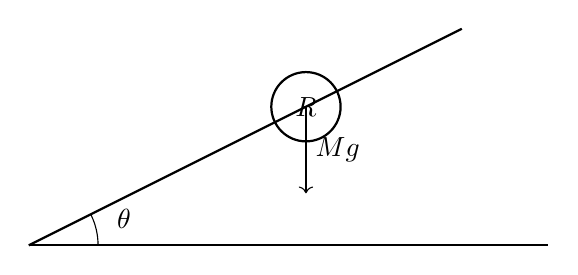
\begin{tikzpicture}[scale=1.1]

% Incline
\draw[thick] (0,0) -- (5,2.5);
\draw[thick] (0,0) -- (6,0);

% Angle marking (correct geometric construction)
\draw (0.8,0) arc (0:26.565:0.8);
\node at (1.1,0.3) {$\theta$};

% Sphere
\draw[thick] (3.2,1.6) circle (0.4);
\node at (3.2,1.6) {$R$};

% Gravity arrow
\draw[->] (3.2,1.6) -- (3.2,0.6);
\node[right] at (3.2,1.1) {$Mg$};

\end{tikzpicture}
\end{center}

A) \(\frac{5g\sin\theta}{7}\left(1-\frac{2\epsilon}{7}\right)\)  

B) \(\frac{5g\sin\theta}{7}\left(1-\frac{\epsilon}{7}\right)\)  

C) \(\frac{5g\sin\theta}{7}\left(1+\frac{2\epsilon}{7}\right)\)  

D) \(\frac{5g\sin\theta}{7}\left(1-\frac{3\epsilon}{14}\right)\)  

---

\item A uniform disc of mass \(M\) and radius \(R\) rotates freely with angular speed \(\omega\) about its central axis; a particle of mass \(m\) approaches tangentially with speed \(v=\omega R\) and sticks at the rim, and no external torque acts about the centre. Considering simultaneous conservation of angular momentum and inelastic energy redistribution, the final angular speed is  

% Diagram for Question 4

\begin{center}
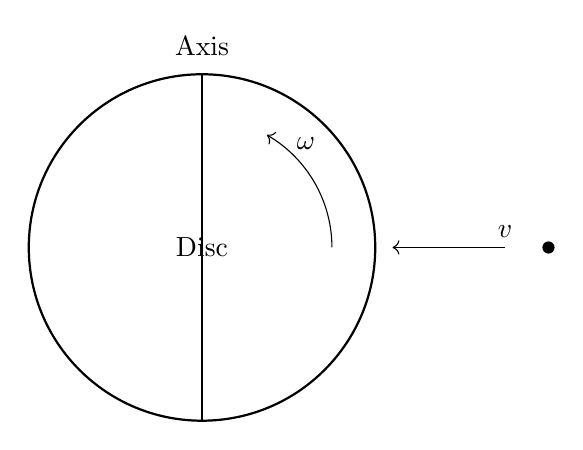
\begin{tikzpicture}[scale=1.1]

% Disc
\draw[thick] (0,0) circle (2);
\node at (0,0) {Disc};

% Axis
\draw[thick] (0,-2) -- (0,2);
\node[above] at (0,2.1) {Axis};

% Angular velocity arrow
\draw[->] (1.5,0) arc (0:60:1.5);
\node at (1.2,1.2) {$\omega$};

% Incoming particle
\fill (4,0) circle (2pt);
\draw[->] (3.5,0) -- (2.2,0);
\node[above] at (3.5,0) {$v$};

\end{tikzpicture}
\end{center}

A) \(\frac{2M}{2M+m}\omega\)  

B) \(\frac{M}{M+m}\omega\)  

C) \(\frac{2M+m}{2M+2m}\omega\)  

D) \(\frac{2M}{2M+3m}\omega\)  

---

\item A satellite of mass \(m\) moves in a circular orbit of radius \(r=3R_E\) around Earth; due to a brief radial inward impulse that does no work but changes angular momentum slightly by fractional amount \(\delta\) (\(|\delta|\ll1\)), it transitions to a nearby circular orbit. To first order in \(\delta\), the fractional change in total mechanical energy is  

A) \(2\delta\)  

B) \(-2\delta\)  

C) \(\delta\)  

D) \(-\delta\)  

---

\item A planet has the same radius as Earth but uniform density \(2\rho_E(1+\epsilon)\), where \(|\epsilon|\ll1\); neglecting rotation and atmosphere, and keeping first order in \(\epsilon\), the escape velocity in terms of Earth’s escape velocity \(v_E\) is  

A) \(\sqrt{2}\,v_E\left(1+\frac{\epsilon}{2}\right)\)  

B) \(\sqrt{2}\,v_E(1+\epsilon)\)  

C) \(\sqrt{2}\,v_E\left(1-\frac{\epsilon}{2}\right)\)  

D) \(2v_E(1+\epsilon)\)  

---

\item A thin spherical shell of mass \(M\) and radius \(R\) has a small circular hole at one point; a particle of mass \(m\) placed just inside the shell along a diameter performs small oscillations under gravitational attraction of the shell only. Using superposition and retaining first-order correction due to missing mass equivalent to a point mass at centre subtending small solid angle \(\Omega\), the angular frequency of oscillation is  

% Diagram for Question 7

\begin{center}
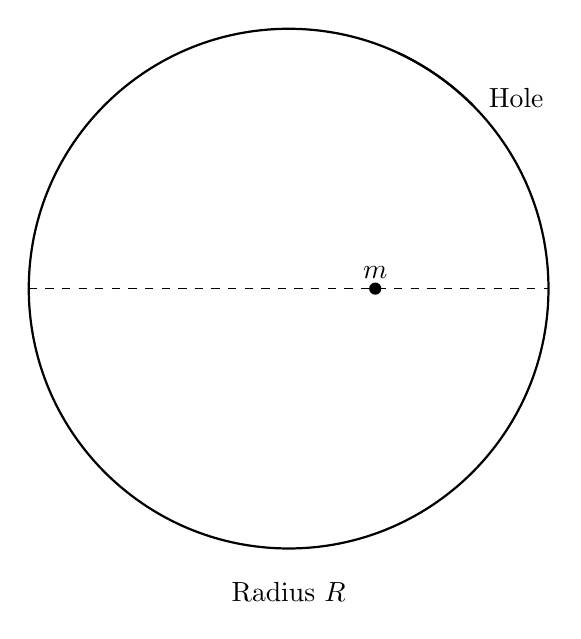
\begin{tikzpicture}[scale=1.1]

% Spherical shell cross-section
\draw[thick] (0,0) circle (3);

% Diameter
\draw[dashed] (-3,0) -- (3,0);

% Particle inside
\fill (1,0) circle (2pt);
\node[above] at (1,0) {$m$};

% Small hole indication (correctly on boundary)
\draw[thick] (45:3) arc (45:65:3);
\node[right] at (2.2,2.2) {Hole};

\node at (0,-3.5) {Radius $R$};

\end{tikzpicture}
\end{center}

A) \(\sqrt{\frac{g}{R}}\left(1-\frac{\Omega}{8\pi}\right)\)  

B) \(\sqrt{\frac{g}{R}}\left(1-\frac{\Omega}{4\pi}\right)\)  

C) \(\sqrt{\frac{g}{R}}\left(1+\frac{\Omega}{8\pi}\right)\)  

D) \(\sqrt{\frac{g}{R}}\left(1-\frac{\Omega}{2\pi}\right)\)  

---

\item A wire of original length \(L\), cross-sectional area \(A\), and Young’s modulus \(Y\) is stretched by a force that increases linearly from 0 to \(F\); accounting for gradual change in length during loading and neglecting higher-order strain terms, the elastic energy stored per unit volume is  

A) \(\frac{F^2}{2AY}\)  

B) \(\frac{F^2}{AY}\)  

C) \(\frac{F^2}{4AY}\)  

D) \(\frac{F^2}{3AY}\)  

---

\item A light circular ring of mass \(M\) rotates with angular velocity \(\omega_0\) about its central axis; a small bead of mass \(m\) initially at centre is pushed radially outward slowly along a spoke to the rim without external torque. If the bead experiences negligible friction with spoke but remains constrained to rotate with ring, the final angular velocity is  

% Diagram for Question 9

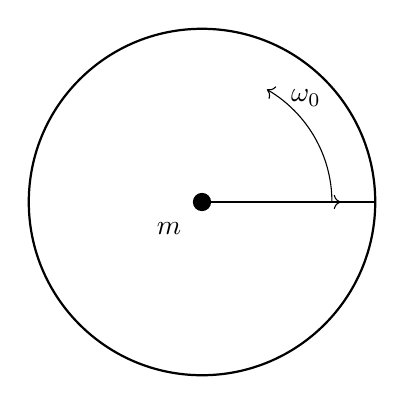
\begin{tikzpicture}[scale=1.1]

% Ring
\draw[thick] (0,0) circle (2);

% Spoke
\draw[thick] (0,0) -- (2,0);

% Bead at centre
\fill (0,0) circle (3pt);
\node[below left=4pt] at (0,0) {$m$};

% Arrow outward
\draw[->] (0.5,0) -- (1.6,0);

% Angular velocity
\draw[->] (1.5,0) arc (0:60:1.5);
\node at (1.2,1.2) {$\omega_0$};

\end{tikzpicture}

A) \(\omega_0\frac{M}{M+m}\)  

B) \(\omega_0\frac{M}{M+2m}\)  

C) \(\omega_0\frac{M+m}{M}\)  

D) \(\omega_0\frac{M}{M+\frac{m}{2}}\)  

---

\item A rigid body has equal principal moments \(I\) about all axes through its centre; a constant torque \(\vec{\tau}\) is applied along a direction fixed in space but not aligned with initial angular velocity. Using Euler’s rotational equation for symmetric body, the angular acceleration vector is  

A) \(\dfrac{\vec{\tau}}{I}\)  

B) \(\dfrac{\vec{\tau}\times\vec{\omega}}{I}\)  

C) \(\dfrac{\vec{\omega}\times\vec{\tau}}{I}\)  

D) Zero  

---

\item A solid cylinder rolls without slipping on a horizontal surface while a constant horizontal force is applied at its centre; static friction adjusts to maintain rolling and the point of contact has zero instantaneous velocity. The work done by static friction over finite displacement is zero because the displacement of point of application relative to ground is  

A) Zero at each instant  

B) Equal to centre displacement  

C) Opposite to motion  

D) Proportional to angular acceleration  

---

\item The gravitational potential inside a uniform thin spherical shell is constant; if a small mass \(m\) is placed anywhere inside, the net gravitational force due to the shell is zero because vector contributions over solid angle satisfy  

A) Exact cancellation by symmetry  

B) Radial enhancement  

C) Tangential dominance  

D) Divergent integral  

---

\item The moment of inertia of a rigid body about two parallel axes separated by distance \(d\) differs by \(Md^2\) because kinetic energy in pure rotation depends on square of perpendicular distance of each mass element from  

A) Instantaneous axis  

B) Centre of mass only  

C) Surface  

D) Density gradient  

---

\item For a satellite in circular orbit under inverse-square gravity, total mechanical energy equals \(-\frac{1}{2}\frac{GMm}{r}\); if orbital radius is decreased infinitesimally while maintaining circular motion, kinetic energy changes such that  

A) It increases in magnitude  

B) It decreases to zero  

C) It remains constant  

D) It becomes negative  

---

\item Within elastic limit, stress is proportional to strain because intermolecular restoring force for small displacement can be approximated as linear in displacement; this corresponds mechanically to potential energy varying approximately as  

A) Square of extension  

B) Linear in extension  

C) Inverse extension  

D) Independent of extension  

\end{enumerate}

\end{document}